\documentclass[tikz,border=2pt]{standalone}
\usepackage{amsmath}
\usetikzlibrary{arrows.meta}
\begin{document}
% if / else if / else chain for one number x: is.na(x) is tested first, then x > 0;
% exactly one result box is reached (NA -> 0, 2 -> 4, -3 -> 3).
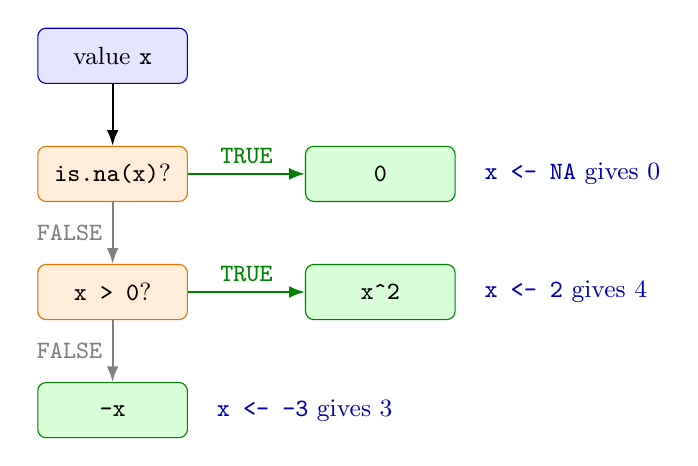
\begin{tikzpicture}[font=\small, >={Latex[length=2mm]},
  box/.style={draw, rounded corners=3pt, minimum height=7mm, minimum width=1.9cm, align=center, inner sep=3pt},
  inp/.style={box, fill=blue!10, draw=blue!70!black},
  test/.style={box, fill=orange!15, draw=orange!90!black},
  res/.style={box, fill=green!15, draw=green!50!black}]
  \node[inp]  (in) at (0,0)    {value \texttt{x}};
  \node[test] (t1) at (0,-1.5) {\texttt{is.na(x)}?};
  \node[test] (t2) at (0,-3.0) {\texttt{x > 0}?};
  \node[res]  (r3) at (0,-4.5) {\texttt{-x}};
  \node[res]  (r1) at (3.4,-1.5) {\texttt{0}};
  \node[res]  (r2) at (3.4,-3.0) {\texttt{x\^{}2}};
  \draw[->, thick] (in) -- (t1);
  \draw[->, thick, gray] (t1) -- node[left, font=\small\ttfamily] {FALSE} (t2);
  \draw[->, thick, gray] (t2) -- node[left, font=\small\ttfamily] {FALSE} (r3);
  \draw[->, thick, green!50!black] (t1) -- node[above, font=\small\ttfamily] {TRUE} (r1);
  \draw[->, thick, green!50!black] (t2) -- node[above, font=\small\ttfamily] {TRUE} (r2);
  \node[anchor=west, blue!70!black] at (4.6,-1.5) {\texttt{x <- NA} gives 0};
  \node[anchor=west, blue!70!black] at (4.6,-3.0) {\texttt{x <- 2} gives 4};
  \node[anchor=west, blue!70!black] at (1.2,-4.5) {\texttt{x <- -3} gives 3};
\end{tikzpicture}
\end{document}
